\documentclass[border=4pt]{standalone}

\usepackage{amsmath}
\usepackage{tikz}
\usepackage{mathdots}
\usepackage{yhmath}
\usepackage{cancel}
\usepackage{color}
\usepackage{siunitx}
\usepackage{array}
\usepackage{multirow}
\usepackage{amssymb}
\usepackage{gensymb}
\usepackage{tabularx}
\usepackage{booktabs}
\usetikzlibrary{fadings}
\usetikzlibrary{patterns}


\begin{document}
 


\tikzset{every picture/.style={line width=0.75pt}} %set default line width to 0.75pt        

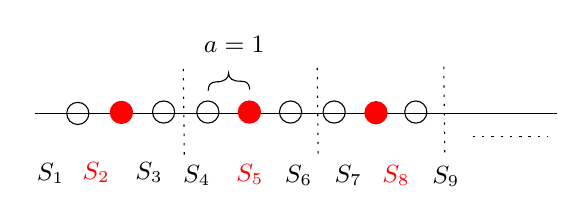
\begin{tikzpicture}[x=0.75pt,y=0.75pt,yscale=-1,xscale=1]
%uncomment if require: \path (0,440); %set diagram left start at 0, and has height of 440

%Straight Lines [id:da10088645641501937] 
\draw    (98,118) -- (349.5,118) ;


%Shape: Circle [id:dp3959942068182474] 
\draw   (113.33,118) .. controls (113.33,115.05) and (115.72,112.67) .. (118.67,112.67) .. controls (121.61,112.67) and (124,115.05) .. (124,118) .. controls (124,120.95) and (121.61,123.33) .. (118.67,123.33) .. controls (115.72,123.33) and (113.33,120.95) .. (113.33,118) -- cycle ;
%Shape: Circle [id:dp4560847301720734] 
\draw   (154.67,117.33) .. controls (154.67,114.39) and (157.05,112) .. (160,112) .. controls (162.95,112) and (165.33,114.39) .. (165.33,117.33) .. controls (165.33,120.28) and (162.95,122.67) .. (160,122.67) .. controls (157.05,122.67) and (154.67,120.28) .. (154.67,117.33) -- cycle ;
%Shape: Circle [id:dp19037510211219044] 
\draw   (176,117.33) .. controls (176,114.39) and (178.39,112) .. (181.33,112) .. controls (184.28,112) and (186.67,114.39) .. (186.67,117.33) .. controls (186.67,120.28) and (184.28,122.67) .. (181.33,122.67) .. controls (178.39,122.67) and (176,120.28) .. (176,117.33) -- cycle ;
%Shape: Circle [id:dp0771192538724692] 
\draw   (215.83,117.33) .. controls (215.83,114.39) and (218.22,112) .. (221.17,112) .. controls (224.11,112) and (226.5,114.39) .. (226.5,117.33) .. controls (226.5,120.28) and (224.11,122.67) .. (221.17,122.67) .. controls (218.22,122.67) and (215.83,120.28) .. (215.83,117.33) -- cycle ;
%Shape: Circle [id:dp7563218202024968] 
\draw   (236.83,117.33) .. controls (236.83,114.39) and (239.22,112) .. (242.17,112) .. controls (245.11,112) and (247.5,114.39) .. (247.5,117.33) .. controls (247.5,120.28) and (245.11,122.67) .. (242.17,122.67) .. controls (239.22,122.67) and (236.83,120.28) .. (236.83,117.33) -- cycle ;
%Shape: Circle [id:dp543383136700875] 
\draw   (276.17,117.33) .. controls (276.17,114.39) and (278.55,112) .. (281.5,112) .. controls (284.45,112) and (286.83,114.39) .. (286.83,117.33) .. controls (286.83,120.28) and (284.45,122.67) .. (281.5,122.67) .. controls (278.55,122.67) and (276.17,120.28) .. (276.17,117.33) -- cycle ;
%Shape: Circle [id:dp1413231242534594] 
\draw  [color={rgb, 255:red, 255; green, 0; blue, 0 }  ,draw opacity=1 ][fill={rgb, 255:red, 255; green, 0; blue, 0 }  ,fill opacity=1 ] (134.33,117.5) .. controls (134.33,114.55) and (136.72,112.17) .. (139.67,112.17) .. controls (142.61,112.17) and (145,114.55) .. (145,117.5) .. controls (145,120.45) and (142.61,122.83) .. (139.67,122.83) .. controls (136.72,122.83) and (134.33,120.45) .. (134.33,117.5) -- cycle ;
%Shape: Circle [id:dp8824634678473726] 
\draw  [color={rgb, 255:red, 255; green, 0; blue, 0 }  ,draw opacity=1 ][fill={rgb, 255:red, 255; green, 0; blue, 0 }  ,fill opacity=1 ] (196,117.33) .. controls (196,114.39) and (198.39,112) .. (201.33,112) .. controls (204.28,112) and (206.67,114.39) .. (206.67,117.33) .. controls (206.67,120.28) and (204.28,122.67) .. (201.33,122.67) .. controls (198.39,122.67) and (196,120.28) .. (196,117.33) -- cycle ;
%Shape: Circle [id:dp9218693548908043] 
\draw  [color={rgb, 255:red, 255; green, 0; blue, 0 }  ,draw opacity=1 ][fill={rgb, 255:red, 255; green, 0; blue, 0 }  ,fill opacity=1 ] (257,117.67) .. controls (257,114.72) and (259.39,112.33) .. (262.33,112.33) .. controls (265.28,112.33) and (267.67,114.72) .. (267.67,117.67) .. controls (267.67,120.61) and (265.28,123) .. (262.33,123) .. controls (259.39,123) and (257,120.61) .. (257,117.67) -- cycle ;
%Straight Lines [id:da41660750271145375] 
\draw  [dash pattern={on 0.84pt off 2.51pt}]  (169.5,96.5) -- (170,140.5) ;


%Straight Lines [id:da41594869222995] 
\draw  [dash pattern={on 0.84pt off 2.51pt}]  (234,96) -- (234.5,140) ;


%Straight Lines [id:da3156062903863326] 
\draw  [dash pattern={on 0.84pt off 2.51pt}]  (295,95.5) -- (295.5,139.5) ;


%Straight Lines [id:da1162064199540842] 
\draw  [dash pattern={on 0.84pt off 2.51pt}]  (309,129) -- (345,129) ;


%Shape: Brace [id:dp18665112675669304] 
\draw   (201.5,106.5) .. controls (201.43,103.75) and (200.03,102.42) .. (197.28,102.49) -- (197.28,102.49) .. controls (193.36,102.58) and (191.36,101.26) .. (191.29,98.51) .. controls (191.36,101.26) and (189.44,102.68) .. (185.51,102.78)(187.28,102.73) -- (185.51,102.78) .. controls (182.77,102.85) and (181.43,104.25) .. (181.5,107) ;

% Text Node
\draw (105.5,147) node  [font=\small]  {$S_{1}$};
% Text Node
\draw (127.5,146.5) node  [font=\small,color={rgb, 255:red, 255; green, 0; blue, 0 }  ,opacity=1 ]  {$S_{2}$};
% Text Node
\draw (153,146.5) node  [font=\small]  {$S_{3}$};
% Text Node
\draw (176,148) node  [font=\small]  {$S_{4}$};
% Text Node
\draw (201.5,147.5) node  [font=\small,color={rgb, 255:red, 255; green, 0; blue, 0 }  ,opacity=1 ]  {$S_{5}$};
% Text Node
\draw (225,148) node  [font=\small]  {$S_{6}$};
% Text Node
\draw (249,148) node  [font=\small]  {$S_{7}$};
% Text Node
\draw (272,148) node  [font=\small,color={rgb, 255:red, 255; green, 0; blue, 0 }  ,opacity=1 ]  {$S_{8}$};
% Text Node
\draw (296,148.5) node  [font=\small]  {$S_{9}$};
% Text Node
\draw (194,85) node  [font=\small]  {$a=1$};


\end{tikzpicture}

\end{document}
